\documentclass{beamer}
\usepackage{pgfpages}
\usepackage[LGR,T1]{fontenc}
\usepackage[utf8]{inputenc}
\usepackage[spanish]{babel}
\usepackage{textcomp}
\usepackage{listings}
\lstset{language=c++, xleftmargin=25pt}
%% listings-modelica.cfg
%% Copyright 2014 Martin Sjoelund, Dietmar Winkler
%
% This work may be distributed and/or modified under the
% conditions of the LaTeX Project Public License, either version 1.3
% of this license or (at your option) any later version.
% The latest version of this license is in
%   http://www.latex-project.org/lppl.txt
% and version 1.3 or later is part of all distributions of LaTeX
% version 2005/12/01 or later.
%
% This work has the LPPL maintenance status `maintained'.
%
% The Current Maintainer of this work is Dietmar Winkler
%
% Code repository https://github.com/modelica-tools/listings-modelica
%
% This work consists of the file listings-modelica.cfg

\lstdefinelanguage{modelica}
{
  morekeywords=[1]{
    algorithm,and,annotation,as,assert,block,break,case,class,connect,connector,
    constant,constrainedby,der,discrete,each,else,elseif,elsewhen,encapsulated,
    end,enumeration,equality,equation,expandable,extends,external,failure,final,
    flow,for,function,guard,if,import,in,initial,inner,input,List,local,loop,
    match,matchcontinue,model,not,operator,Option,or,outer,output,package,parameter,
    partial,protected,public,record,redeclare,replaceable,return,stream,
    subtypeof,then,Tuple,type,uniontype,when,while},
  morekeywords=[2]{true, false},
  % Do not make true,false keywords because fn(true,x, false ) shows up as fn(true,x, *false*)
  sensitive=true,
  comment=[l]//,
  morecomment=[s]{/*}{*/},
  alsodigit={.,-},
  morestring=[b]',
  morestring=[b]",
}[keywords,comments,strings]

\definecolor{keywordcolor1}{rgb}{0,0,.4}
\definecolor{keywordcolor2}{rgb}{.90,0,0}
\definecolor{stringcolor}{rgb}{0.133,0.545,0.133}
% \definecolor{listingbgcolor}{rgb}{0.95,0.95,0.95}

\lstset{
  breaklines=true,
  language=modelica,
  basicstyle=\ttfamily,
  keywordstyle=[1]\color{keywordcolor1}\bfseries,
  keywordstyle=[2]\color{keywordcolor2},
  stringstyle=\color{stringcolor},
%  backgroundcolor=\color{listingbgcolor},
  framexleftmargin=5pt,
  xleftmargin=5pt,
  xrightmargin=5pt,
  showstringspaces=false,
}

\lstset{breaklines=true,label=}
% \lstset{basicstyle=\ttfamily}

\newcommand{\code}[1]{\texttt{\hyphenchar%
\font45%
\sloppy%
\fontdimen2\font=0.4em%
\fontdimen3\font=0.2em%
\fontdimen4\font=0.1em%
\fontdimen7\font=0.1em%
 #1}}

\usepackage{amsmath}
\usepackage{mathtools}
\DeclarePairedDelimiter{\abs}{\lvert}{\rvert}
\usepackage{float}
\usepackage{graphicx}
\usepackage{caption}
\usepackage{subcaption}
\usepackage{epstopdf}

\setbeameroption{show notes on second screen}

\usetheme{Madrid}

 \AtBeginSection[]
{
  \begin{frame}
    \frametitle{Table of Contents}
    \tableofcontents[currentsection]
  \end{frame}
}
 
\title[] %optional
{Causalización de Modelos Modelica}
 
\subtitle{Tesina de Grado}
 
\author[] % (optional, for multiple authors)
{Federico~Moya}
 
\institute[] % (optional)	
{
  Licenciatura en Cs. de la Computación\\
  Facultad de Cs. Exactas, Ingeniería y Agrimensura\\
  Universidad Nacional de Rosario
}
 
\date[] % (optional)
{Agosto 2016}
 
% \logo{
\includegraphics[height=1.5cm]{graphics/logo_unr.jpg}}
 
\begin{document}
 
\section{Contexto}

\begin{frame}{Contexto}
    \begin{itemize}
        \item<1-> Proyecto de investigación de la U.N.R: Modelado, Simulación y Control en Tiempo Real con Aplicaciones en Electrónica de Potencia.
        \item<2-> Desarrollar un compilador Modelica con los fines de investigar distintos algoritmos en relación a modelos de gran escala.
        \item<3-> Causalización de ecuaciones diferenciales algebraicas mediante la aplicación del algoritmo de Tarjan.
    \end{itemize}
\end{frame}

\section{Modelado y Simulación}

\begin{frame}{Sistema y Experimento}
	\begin{itemize}
        \item<1-> Un sistema es un objeto o una colección de objetos cuyas propiedades queremos estudiar.
	  	\item<2-> Para un sistema se pueden definir variables de entrada y variables de salida.
        \note{
            \begin{itemize}
                \item Las entradas son variables del entorno que influencian el comportamiento del sistema. Estas entradas pueden o no ser controlables por nosotros. 
                \item Las salidas de un sistema son variables que son determinadas por el sistema y pueden influenciar el entorno que lo rodea.
            \end{itemize}
        }
        \item<3-> Un experimento es el proceso de extraer información de un sistema ejercitando sus entradas.
        \note{
            Desventajas del método experimental:
                \begin{itemize}
                    \item Para un gran número de sistemas muchas variables de entrada no son accesibles ni controlables.
                    \item Algunas variables de salida importantes no resultan accesibles para poder medirlas; estas variables a veces se denominan estados internos del sistema.
                    \item Problemas prácticos (el experimento puede ser muy caro, o peligroso, o bien el sistema necesario para el experimento puede que todavía no exista).
                \end{itemize}
        }
	\end{itemize}
\end{frame}

\begin{frame}{Modelado y Simulación}
    \begin{itemize}
        \item<1-> Un modelo de un sistema es cualquier cosa sobre la cual se puede aplicar un “experimento” con el objeto de responder preguntas sobre el sistema.
    	\item<2-> Un modelo matemático es una descripción de un sistema en donde las relaciones entre las variables se expresan en forma matemática mediante ecuaciones.
        \note{Las variables pueden ser cantidades medibles como tamaño, longitud, peso, temperatura, nivel de desempleo, flujo de información, etc. La mayoría de las leyes de físicas son modelos matemáticos en este sentido.}
        \item<3-> Una simulación es un experimento realizado sobre un modelo.
        \note{
            Algunos ejemplos de simlación:
            \begin{itemize}
                \item<1-> La simulación de un proceso industrial como la producción de acero o papel para aprender sobre el comportamiento bajo diferentes condiciones de operación con el objetivo de mejorar el proceso.
                \item<2-> La simulación del comportamiento de un vehículo, por ejemplo un auto o un avión, para que el conductor o piloto pueda disponer de un entrenamiento realista.
                \item<3-> La simulación de un modelo simplificado de una red de computadoras para aprender cómo se comporta bajo diferentes cargas con el objetivo de mejorar la eficiencia.
            \end{itemize}
        }
    \end{itemize}
\end{frame}

\section{Modelos Matemáticos para Sistemas Continuos}

\begin{frame}{Categorías de variables y constantes}
    \begin{itemize}
        \item<1-> \textbf{Constante:} una cantidad en el modelo que no varía nunca, por ejemplo la gravedad en la tierra $g=9.8$.
        \item<2-> \textbf{Parámetro de modelo:} una constante en el modelo que es determinada por el sistema, o una constante que puede ser modificada con el fin de darle diferentes propiedades al sistema. Permance constante durante la simulación pero puede ser modificado entre ejecuciones.
        \item<3-> \textbf{Variable:} una cantidad en el modelo que varia respecto del tiempo.
    \end{itemize}
\end{frame}

\begin{frame}{Categorías de variables y constantes}
    \begin{itemize}
        \item<1-> \textbf{Variable de salida:} una variable cuyo comportamiento queremos observar. Usualmente denotada como $y(t)$. El rol de variable de salida no está establecido por el sistema que se modela sino que es determinado por lo que el modelador quiere estudiar.
        \item<2-> \textbf{Variable de entrada:} una variable que afecta el comportamiento del modelo sin ser afectada por otras variables del modelo y cuyas variaciones respecto del tiempo pueden ser controladas. Usualmente se las denota $u(t)$.
        \item<3-> \textbf{Variable de estado}: una variable que no es ni de entrada ni de salida y que aparece su derivada respecto del tiempo, usualmente denotada por $\dot{x}(t)$
        \item<4-> \textbf{Variables algebraicas:} una variable que aparece en las ecuaciones pero que su derivada no aparece en el modelo.
    \end{itemize}
\end{frame}

\begin{frame}{Ecuacion diferencial ordinaria en forma de espacio de estados explícita}

    \note{ Las ecuaciones diferenciales ordinarias aparecen en la mayoría de los modelos matemáticos de sistemas continuos dado que la dependencia respecto del tiempo en esos modelos generalmente se refleja por medio de derivadas respecto del tiempo de variables de estado correspondientes a dichos modelos.\\
    Un modelo ODE de espacio de estados explícito resulta más eficiente de resolver y analizar que otros modelos más complicados. }

    \begin{block}{Forma general}
        \begin{align*}
            \dot{x}(t) & =f(x(t),u(t)) \\
            y(t)       & =g(x(t),u(t))
        \end{align*}
    \end{block}
    \begin{block}{Ejemplo: Ley de fuerza de Newton}
        $m\ddot{s}(t)=F(t)$\\
        \pause
        \begin{align*}
            \dot{v}(t) & =\frac{F(t)}{m}\\
            \dot{s}(t) & =v(t)
        \end{align*}
    \end{block}
\end{frame}

\begin{frame}[fragile]{Ecuacion diferencial algebraica}
   \framesubtitle{Ejemplo: Péndulo Plano} 
    \note{Cinco de las ecuaciones del modelo son diferenciales y dos son algebraicas.
        Las variables del modelo son $x$, $y$, $v_{x}$, $v_{y}$, $\varphi$,
        $\omega$, $F$ y las constantes $L$, $m$, $g$. Hemos reemplazado
        la ecuación correspondiente a la ley de Pitagóras por dos ecuaciones
        algebraicas sobre las variables $x$ e $y$ respectivamente, las cuales
        aún preservan la restricción sobre la longitud del péndulo.}
    \begin{columns}
        \begin{column}{0.5\textwidth}
            \begin{figure}
              \centering
              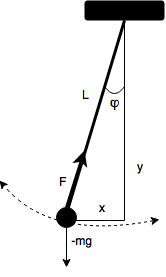
\includegraphics[width=0.5\textwidth]{graphics/pendulum.png}
            \end{figure}
        \end{column}
        \begin{column}{0.5\textwidth}
            \begin{align*}
                m\dot{v_{x}}  & =-F\sin(\varphi)\nonumber \\
                m\dot{v_{y}}  & =-F\cos(\varphi)-mg\nonumber \\
                \dot{x}       & =v_{x}\nonumber \\
                \dot{y}       & =v_{y}\label{eq:pendulo}\\
                \dot{\varphi} & =\omega\nonumber \\
                x             & =L\sin(\varphi)\nonumber \\
                y             & =-L\cos\left(\varphi\right)\nonumber
            \end{align*} 
        \end{column}
    \end{columns}
\end{frame}

\begin{frame}[fragile]{Ecuacion diferencial algebraica}
   
   \note{ Las ecuaciones diferenciales algebraicas no son los modelos más eficientes para resolver ya que las derivadas no siempre aparecen del lado izquierdo y por lo tanto puede ser necesario aplicar derivación numérica }

   \begin{block}{Forma General}
       \begin{align*}
            F(x(t),\dot{x}(t),u(t),y(t)) & =0 \\
            G(x(t),u(t),y(t))            & =0
       \end{align*}
    \end{block}
\end{frame}






\section{Modelica}

\begin{frame}{Modelica}
    \begin{block}<1->{}
        Es un lenguaje de modelado (estándar abierto) que permite la especificación de modelos matemáticos de complejos sistemas naturales o artificiales.
    \end{block}
    Características principales:
    \begin{itemize}
        \item<2-> Modelica es un lenguaje orientado a objetos con un concepto general de clase que unifica las ideas de clases, tipos genéricos y subtipos en un solo lenguaje. Esto facilita la reutilización de componentes y la evolución de los modelos. 
    \end{itemize}
\end{frame}

\begin{frame}{Modelica}
    \begin{itemize}
        \item<1-> Modelica está principalmente basado en ecuaciones en lugar de asignaciones. Esto permite un modelado acausal lo cual facilita la reutilización de las clases ya que las ecuaciones no especifican una dirección particular para el flujo de datos. De esta manera una clase Modelica se puede adaptar a contextos con diferentes flujos de datos.
        \item<2-> Modelica permite describir y conectar componentes de modelos pertenecientes a diferentes dominios como eléctricos, mecánicos, termodinámica, hidráulica, biología, control, etc. 
    \end{itemize}
\end{frame}

\begin{frame}{Conceptos básicos}
    \begin{itemize}
        \item<1-> Un modelo Modelica se construye a partir de clases.
        \item<2-> Los principales elementos que contiene una clase  son declaraciones de variables y ecuaciones.
    \end{itemize}
\end{frame}

\begin{frame}[fragile]{Conceptos básicos}
   \framesubtitle{Ejemplo: Péndulo Plano}
   \fontsize{8pt}{7.2}\selectfont
    \begin{columns}
    % \begin{minipage}[t]{2cm}
        \begin{column}{0.4\textwidth}
                \begin{align*}
                    m\dot{v_{x}}  & =-F\sin(\varphi)\nonumber \\
                    m\dot{v_{y}}  & =-F\cos(\varphi)-mg\nonumber \\
                    \dot{x}       & =v_{x}\nonumber \\
                    \dot{y}       & =v_{y}\\
                    \dot{\varphi} & =\omega\nonumber \\
                    x             & =L\sin(\varphi)\nonumber \\
                    y             & =-L\cos\left(\varphi\right)\nonumber
                \end{align*}
        \end{column}
        % \end{minipage}
        \begin{column}{0.6\textwidth}
        % \begin{minipage}[t]{10cm}
            \begin{lstlisting}[language=Modelica]
class Pendulum "Planar Pendulum"
  parameter Real m=1, g=9.81, L=O.5;
  Real F, phi, omega;
  output Real x(start=O.5);
  output Real y(start=O);
  output Real vx,vy;
  equation
    m*der(vx)=-F*sin(phi);
    m*der(vy)=-F*cos(phi)-m*g;
    der(x)=vx;
    der(y)=vy;
    der(phi)=omega;
    x=L*sin(phi);
    y=-L*cos(phi);
end Pendulum;
            \end{lstlisting}
        % \end{minipage}
        \end{column}
    \end{columns}
\end{frame}

\begin{frame}[fragile]{Modelado acausal}
    La ecuación característica de una resistencia, $Ri=v$, puede utilizarse de diferentes maneras.
    \pause
    \begin{itemize}
        \item<1-> Para calcular la corriente a partir del voltaje y de la resistencia: $i :=\frac{v}{R}$
        \item<2-> Para calcular el voltaje a partir de la resistencia
y de la corriente: $v :=R\times i$
        \item<3-> Para calcular la resistencia a partir del voltaje y
de la corriente: $R :=\frac{v}{i}$
    \end{itemize}
\end{frame}

\begin{frame}{Compilación y Ejecución de Modelos Modelica}
    \note{Análisis sintáctico del código fuente Modelica del cual se obtiene un árbol sintáctico abstracto. Se analiza gramaticalmente, se realiza la verificación de tipos, las clases se heredan y expanden, las ecuaciones connect se convierten en ecuaciones comunes,
etc. El resultado de este proceso de análisis y traducción es un conjunto plano de ecuaciones, constantes, variables y funciones. No queda ningún rastro de la estructura de objetos.
Luego un módulo de optimización compuesto por algoritmos de simplificación algebraica, métodos de
reducción de índices, etc., elimina la mayoría de las ecuaciones dejando solo un conjunto mínimo que eventualmente va a ser resuelto numéricamente. Por ejemplo, si dos variables son sintácticamente equivalentes solo
se conserva una.
Causalización.
Finalmente se genera código en algún lenguaje de programación convencional,
usualmente C, y se lo enlaza con algún método de integración numérica.
}
    \begin{figure}[H]
      \centering
      \includegraphics[width=1\textwidth]{graphics/compilacion_ejecucion_modelica.png}
    \end{figure}
\end{frame}

 
\section{Causalización de un sistema DAE}

\begin{frame}{Causalización}
    ¿Como convertimos un modelo DAE acausal en un modelo ODE causalizado?
    \pause
    \begin{itemize}
        \item<2-> Necesitamos reordenar horizontalmente el modelo de manera que del lado izquierdo de cada ecuación solo aparezca o bien la derivada de una variable de estado o bien una variable algebraica.
        \item<3-> Necesitamos ordenar verticalmente las ecuaciones de manera que puedan ser resueltas secuencialmente.
    \end{itemize}
\end{frame}

\begin{frame}{Causalización}
    \begin{itemize}
        \item<1-> Definimos que para toda variable $x$ tal que $\dot{x}$ aparece en el modelo, $x$ es conocida y $\dot{x}$ es una incógnita.
        \item<2-> Construimos un grafo bipartito no dirigido a partir del modelo DAE.
        \item<3-> Calculamos un matching máximo sobre el grafo para definir qué variable vamos a despejar de qué ecuación.
        \item<4-> A partir del grafo bipartito y del matching construimos un grafo dirigido.
        \item<5-> Aplicamos el algoritmo de Tarjan sobre el grafo dirigido. De esta manera obtenemos un orden para las ecuaciones del sistema.
    \end{itemize}
\end{frame}

\begin{frame}{Algoritmo de Tarjan}
    \begin{itemize}
        \item<1-> Permite encontrar los componentes fuertemente conexos en un grafo dirigido.
        \item<2-> Complejidad $O(\abs{V}+\abs{E})$
        \item<3-> Posee la propiedad de que ningún componente fuertemente conexo va a ser identificado antes que alguno de sus sucesores. De esta manera el orden en el que son identificados los componentes fuertemente conexos constituye un orden topológico reverso del grafo dirigido acíclico formado por los mismos componentes fuertemente conexos.
    \end{itemize}
\end{frame}

\begin{frame}{Algoritmo de Tarjan}
    \framesubtitle{Ejemplo}
    \begin{figure}
        \includegraphics[width=0.6\textwidth]{graphics/tarjan_step_0.png}
    \end{figure}
\end{frame}

\begin{frame}{Algoritmo de Tarjan}
    \framesubtitle{Ejemplo}
    \begin{figure}
        \includegraphics[width=0.7\textwidth]{graphics/tarjan_step_1.png}
    \end{figure}
\end{frame}

\begin{frame}{Algoritmo de Tarjan}
    \framesubtitle{Ejemplo}
    \begin{figure}
        \includegraphics[width=0.7\textwidth]{graphics/tarjan_step_2.png}
    \end{figure}
\end{frame}

\begin{frame}{Algoritmo de Tarjan}
    \framesubtitle{Ejemplo}
    \begin{figure}
        \includegraphics[width=0.7\textwidth]{graphics/tarjan_step_3.png}
    \end{figure}
\end{frame}

\begin{frame}{Algoritmo de Tarjan}
    \framesubtitle{Ejemplo}
    \begin{figure}
        \includegraphics[width=0.7\textwidth]{graphics/tarjan_step_4.png}
    \end{figure}
\end{frame}


\begin{frame}[fragile]{Aplicación del Algoritmo de Tarjan sobre un modelo DAE}
    \begin{columns}
        \begin{column}{0.5\textwidth}
          \centering
          \begin{align*}
            f_1(z_3,z_4) &= 0 \\
            f_2(z_2) &= 0 \\
            f_3(z_2,z_3,z_5) &= 0 \\
            f_4(z_1,z_2) &= 0 \\
            f_5(z_1,z_3,z_5) &= 0 \\
          \end{align*}
        \end{column}
        \begin{column}{0.5\textwidth}
        \begin{figure}
           \centering
           \includegraphics[width=0.8\textwidth]{graphics/bipartito_original.png}
        \end{figure}
        \end{column}
    \end{columns}
\end{frame}

\begin{frame}[fragile]{Aplicación del Algoritmo de Tarjan sobre un modelo DAE}
    \begin{columns}
        \begin{column}{0.5\textwidth}
        \begin{figure}
           \centering
           \includegraphics[width=0.6\textwidth]{graphics/bipartito_matching.png}
        \end{figure}
        \end{column}
        \begin{column}{0.5\textwidth}
        \begin{figure}
           \centering
           \includegraphics[width=0.8\textwidth]{graphics/dirigido.png}
        \end{figure}
        \end{column}
    \end{columns}
\end{frame}

\begin{frame}[fragile]{Aplicación del Algoritmo de Tarjan sobre un modelo DAE}
    \begin{columns}
        \begin{column}{0.5\textwidth}
            \begin{figure}
               \centering
               \includegraphics[width=0.8\textwidth]{graphics/dirigido_componentes.png}
            \end{figure}
        \end{column}  
        \begin{column}{0.5\textwidth}
            \begin{align*}
            f_2(z_2) &= 0 \\
            f_4(z_1,z_2) &= 0 \\
            \mathbf{f_3(z_2,z_3,z_5)} &= \mathbf{0} \\ 
            \mathbf{f_5(z_1,z_3,z_5)} &= \mathbf{0} \\
            f_1(z_3,z_4) &= 0 \\
            \end{align*}
        \end{column}
    \end{columns}
\end{frame}


% \section{Visión General del Compilador ModelicaCC}

\begin{frame}
    La compilación de un modelo Modelica es el proceso mediante el cual se transforma un modelo de alto nivel, el cual puede contener clases y ecuaciones acausales, en un modelo plano, sin clases, y donde las ecuciones se encuentran ordenadas o causalizadas.
    \pause
    El compilador ModelicaCC se planteo como un conjunto de componentes independientes.
    \pause
    \begin{itemize} 
        \item<1-> \textbf{flatter}: Es el componente encargado de el análisis sintáctico y semántico, y del aplanado de la estructura de objetos. 
        \item<2-> \textbf{μModelica}: Es el componente responsable de reescribir el modelo utilizando un subconjunto del lenguaje Modelica denominado μModelica.
        \item<3-> \textbf{antialias}: Es el componente encargado de eliminar ecuaciones triviales de la forma \verb+a=b+.
        \item<4-> \textbf{cauzalize} Es el componente responsable de la causalización del conjunto de ecuaciones del modelo.
\end{frame}

\end{document}
